\documentclass[border=4pt]{standalone}
\usepackage{fontspec}
\usepackage{amsmath}
\usepackage{unicode-math}
\setmainfont{Latin Modern Roman}
\setmathfont{Latin Modern Math}
\usepackage{pgfplots}
\usepackage{pgfplotstable}
\pgfplotsset{compat=1.18}
\usepackage{tkz-euclide}
\usetikzlibrary{arrows.meta,calc,angles,quotes,patterns,3d,backgrounds}
\definecolor{ink}{HTML}{123428}
\definecolor{asy}{HTML}{475569}
\definecolor{mint}{HTML}{86e0bd}
\tikzset{asym/.style={asy, line width=0.9pt, dash pattern=on 5pt off 3.5pt},
         guide/.style={gray!70, line width=0.6pt, densely dotted},
         dot/.style={circle, inner sep=0pt, minimum size=5pt, draw=white, line width=0.5pt},
         odot/.style={circle, inner sep=0pt, minimum size=5.5pt, fill=white, line width=1pt},
         lab/.style={font=\footnotesize, inner sep=1.5pt, text=ink}}
\begin{document}
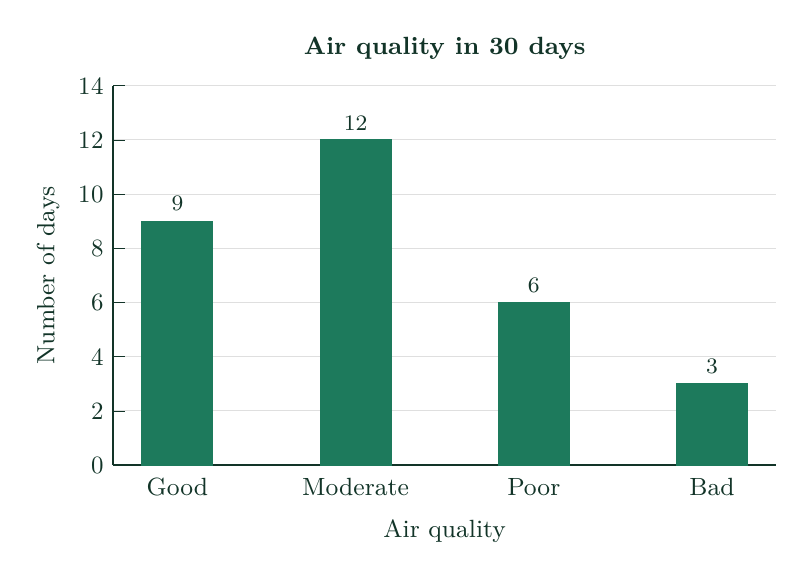
\begin{tikzpicture}
\begin{axis}[width=10cm, height=6.4cm, ymin=0, ymax=14, ytick distance=2, ymajorgrids, grid style={gray!25}, axis lines*=left, axis line style={ink, line width=0.7pt}, tick style={ink}, tick label style={font=\small, text=ink}, xticklabel style={text height=1.7ex, text depth=0.5ex}, xlabel={Air quality}, ylabel={Number of days}, label style={font=\small, text=ink}, title={Air quality in 30 days}, title style={font=\bfseries\small, text=ink}, symbolic x coords={c0,c1,c2,c3}, xtick=data, enlarge x limits=0.12, clip=false, nodes near coords style={font=\footnotesize, text=ink}, xticklabels={{Good},{Moderate},{Poor},{Bad}}, ]
\addplot[ybar, bar width=0.9cm, fill={rgb,255:red,29;green,122;blue,92}, draw={rgb,255:red,29;green,122;blue,92}, ] coordinates {(c0,9) (c1,12) (c2,6) (c3,3)};
\node[font=\footnotesize, text=ink, above] at (axis cs:c0,9) {9};
\node[font=\footnotesize, text=ink, above] at (axis cs:c1,12) {12};
\node[font=\footnotesize, text=ink, above] at (axis cs:c2,6) {6};
\node[font=\footnotesize, text=ink, above] at (axis cs:c3,3) {3};
\end{axis}\end{tikzpicture}
\end{document}
